\documentclass[border=10pt]{standalone}
\usepackage{tikz}
\usetikzlibrary{positioning, trees, calc}
\begin{document}
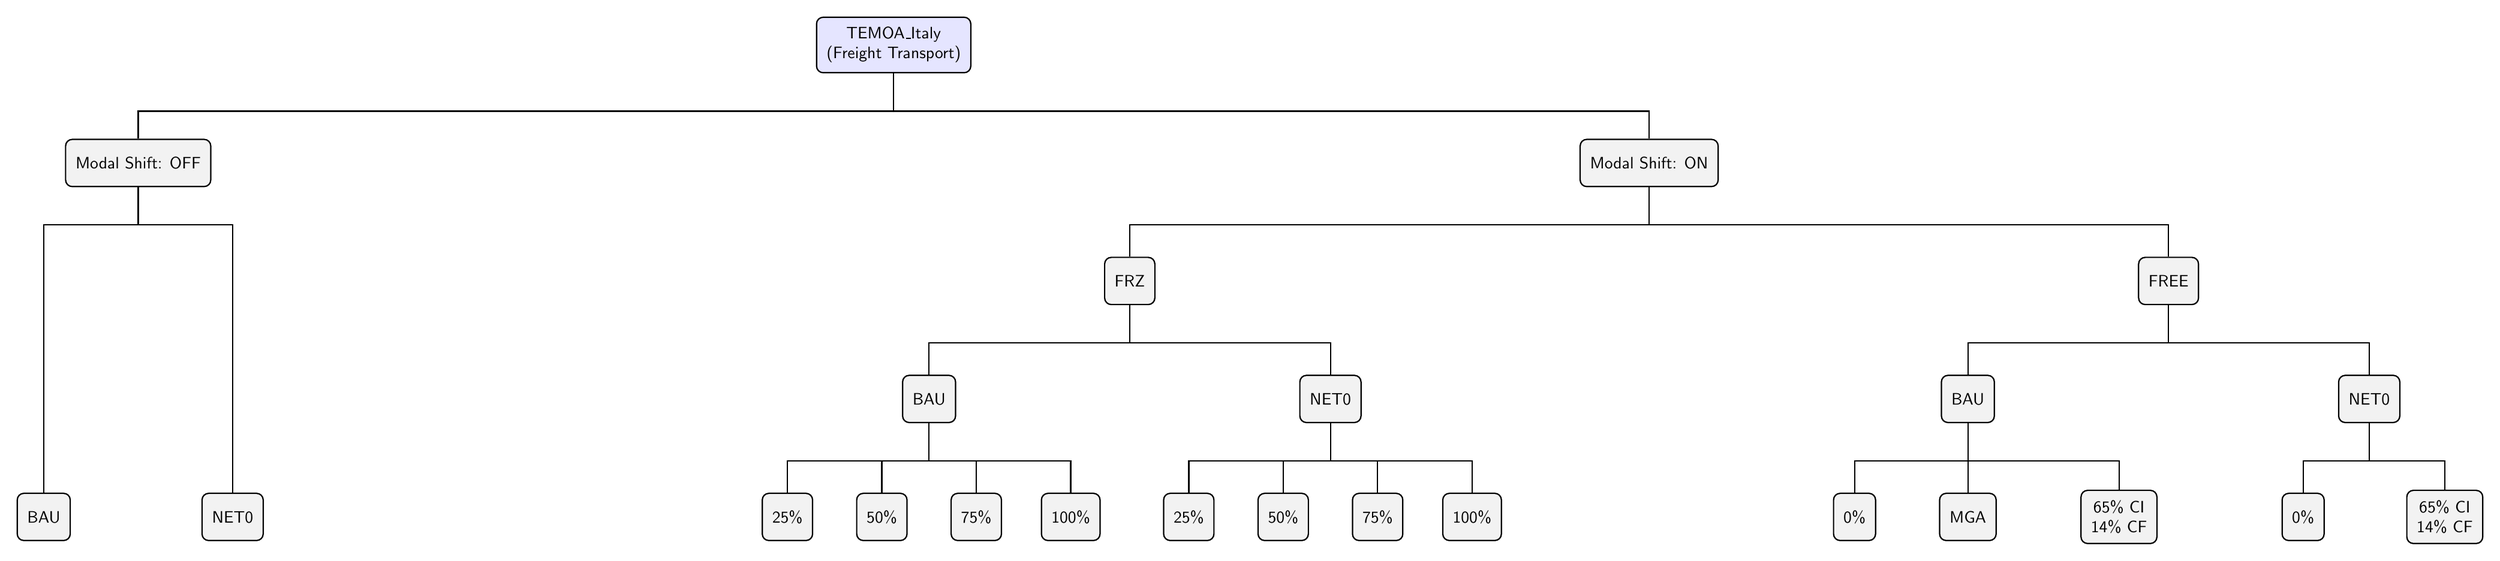
\begin{tikzpicture}[
  level 1/.style={sibling distance=32cm, level distance=2.5cm},
  level 2/.style={sibling distance=22cm, level distance=2.5cm},
  level 3/.style={sibling distance=8.5cm, level distance=2.5cm},
  level 4/.style={sibling distance=2.2cm, level distance=2.5cm},
  every node/.style={shape=rectangle, rounded corners, draw, align=center, fill=gray!10, thick, font=\sffamily, minimum height=1cm, inner sep=6pt},
  edge from parent path={
    (\tikzparentnode.south) -- +(0,-0.8cm) -| (\tikzchildnode.north)
  },
  edge from parent/.style={draw, thick}
]

  \node[fill=blue!10] {TEMOA\_Italy \\ (Freight Transport)}
    child { node {Modal Shift: OFF}
      child[level distance=7.5cm, sibling distance=4cm] { node {BAU} }
      child[level distance=7.5cm, sibling distance=4cm] { node {NET0} }
    }
    child { node {Modal Shift: ON}
      child { node {FRZ}
        child { node {BAU}
          child[sibling distance=2cm] { node {25\%} }
          child[sibling distance=2cm] { node {50\%} }
          child[sibling distance=2cm] { node {75\%} }
          child[sibling distance=2cm] { node {100\%} }
        }
        child { node {NET0}
          child[sibling distance=2cm] { node {25\%} }
          child[sibling distance=2cm] { node {50\%} }
          child[sibling distance=2cm] { node {75\%} }
          child[sibling distance=2cm] { node {100\%} }
        }
      }
      child { node {FREE}
        child { node {BAU}
          child[sibling distance=2.4cm] { node {0\%} }
          child[sibling distance=2.4cm] { node {MGA} }
          child[sibling distance=3.2cm] { node {65\% CI \\ 14\% CF} }
        }
        child { node {NET0}
          child[sibling distance=2.8cm] { node {0\%} }
          child[sibling distance=3.2cm] { node {65\% CI \\ 14\% CF} }
        }
      }
    };

\end{tikzpicture}
\end{document}